\documentclass[journal,10pt]{IEEEtran}

\usepackage[utf8]{inputenc}
\usepackage{amsmath,amssymb,amsfonts}
\usepackage{algorithmic}
\usepackage{graphicx}
\usepackage{textcomp}
\usepackage{xcolor}
\usepackage{booktabs}
\usepackage{multirow}
\usepackage{hyperref}
\usepackage{cite}
\usepackage{url}

\hypersetup{
    colorlinks=true,
    linkcolor=blue,
    filecolor=magenta,      
    urlcolor=cyan,
    citecolor=blue,
}

\begin{document}

\title{SasakNLP: A Dialect-Aware Morphological Processing Framework for the Low-Resource Sasak Language}

\author{\IEEEauthorblockN{kodetr}
\IEEEauthorblockA{\textit{Regional Language Computational Research Group} \\
\textit{kodetr.com}, Lombok, West Nusa Tenggara, Indonesia \\
Correspondence: \url{https://kodetr.com} \\
GitHub: \url{https://github.com/kodetr/sasaknlp}
}}

\maketitle

\begin{abstract}
Bahasa Sasak is an Austronesian regional language spoken by approximately 3 million people across Lombok Island, West Nusa Tenggara (NTB), Indonesia. Despite its demographic vitality, it remains a digitally underrepresented low-resource language lacking standardized computational linguistic infrastructure \cite{aji2022, winata2023}. Standard Indonesian morphological analyzers fail when applied to Sasak due to distinct morphophonemic alternations, complex clitic attachments, and sharp cross-island dialectal variation \cite{hakim2023, yaqin2022, abidin2024}. This paper presents \textbf{SasakNLP}, a dialect-aware morphological processing framework engineered specifically for Sasak orthographic normalization, reduplication-aware tokenization, shibboleth-driven dialect contextualization, and dictionary-validated multi-candidate lemmatization \cite{balaibahasa2022, sasaknlp2026, jurafsky2024}.

Empirical evaluation across an extensive 100,000-pair morphological benchmark and an authentic folklore corpus of 12,591 sentences demonstrates that SasakNLP achieves an overall lemmatization accuracy of \textbf{80.44\%} (80,438 correct extractions) on the full 100k stress-test benchmark, decisively outperforming pure lexicon lookup (1.01\%) and greedy affix-stripping baselines (55.21\%) with strong statistical significance (McNemar's test, $\chi^2 = 14,962.14, p < 0.0001$). On the 10,000-pair core morphological benchmark, the system achieves an accuracy of \textbf{93.23\%}. Error taxonomy analysis confirms that dictionary-gating restricts overstemming to \textbf{2.28\%}, with understemming restricted to \textbf{15.86\%} primarily occurring on complex multi-layered affixations. Computationally, SasakNLP delivers high-throughput execution at \textbf{7,826 words per second} on full 100k batches and up to \textbf{16,272 words per second} on standard sequences, maintaining an average per-token latency of \textbf{0.044 ms} with zero heavy machine learning framework dependencies. All source code, datasets, and interactive web demos are publicly released under permissive open-source licenses \cite{sasaknlp2026}.
\end{abstract}

\begin{IEEEkeywords}
Sasak Language, Natural Language Processing, Computational Morphology, Lemmatization, Low-Resource NLP, Dialectology, Open Science.
\end{IEEEkeywords}

\section{Introduction}
\IEEEPARstart{R}{ecent} breakthroughs in Natural Language Processing (NLP) and Large Language Models (LLMs) have been overwhelmingly concentrated on high-resource languages \cite{aji2022, ranathunga2023}. In Indonesia, while the national language (Bahasa Indonesia) enjoys mature computational infrastructure and pre-trained language representations \cite{cahyawijaya2021indonlg, koto2021}, empirical evaluations indicate that state-of-the-art LLMs suffer catastrophic performance degradation when evaluated on indigenous regional languages and local Indonesian reasoning tasks \cite{koto2023indommlu}. More than 700 indigenous regional languages across Indonesia remain critically neglected and underrepresented \cite{aji2022, winata2023}. This digital resource scarcity creates acute vocabulary mismatch and tokenization fragmentation in downstream NLP pipelines \cite{cahyawijaya2023}, exacerbated by the wide cultural and linguistic nuances across Indonesian provinces \cite{koto2024indoculture}.

Bahasa Sasak (\textit{Basa Sasak}) is the predominant indigenous language of Lombok Island in West Nusa Tenggara, spoken by approximately 3 million native speakers \cite{hakim2023, balaibahasa2022}. Categorized typologically within the Western Malayo-Polynesian branch of the Austronesian language family, Sasak exhibits distinct grammatical and sociopragmatic characteristics \cite{yaqin2022, hakim2022}:
\begin{enumerate}
    \item \textbf{Complex Morphophonemics}: Stem formation incorporates active prefixes (\texttt{te-}, \texttt{ka-}, \texttt{se-}, \texttt{pe-}), archaic passive infixes (\texttt{-in-}, \texttt{-um-}), causative/applicative suffixes (\texttt{-ang}, \texttt{-an}, \texttt{-i}, \texttt{-in}), iterative circumfixes (\texttt{pe-...-an}, \texttt{te-...-ang}, \texttt{be-...-an}), and intricate nasal substitutions ($N$-) \cite{balaibahasa2022, abidin2024}.
    \item \textbf{Enclitic Compounding and Sociopragmatics}: Pronominal possessive enclitics (\texttt{-ku}, \texttt{-m}, \texttt{-ne}) and honorific sociolinguistic particles (\texttt{-de}, \texttt{-te}) append directly to root words, reflecting strict social strata and politeness registers \cite{yaqin2022}, while frequently triggering severe overstemming or understemming in naive heuristic parsers \cite{abidin2024}.
    \item \textbf{Dialectal Diversity}: The language is partitioned into five distinct dialect clusters separated by isoglosses and diagnostic lexical markers (\textit{shibboleths}) \cite{hakim2023, hakim2022}.
\end{enumerate}

Prior computational morphology research in Indonesia has predominantly addressed Javanese and Sundanese \cite{aji2022, abidin2024, wijono2021}, while computational methods for ethnic languages in Eastern Indonesia remain largely confined to bilingual lexicon induction \cite{resiandi2023}. Systematic literature reviews confirm that the absence of structured digital lexicons and morphological analyzers remains the primary barrier to regional language lemmatization \cite{abidin2024}.

To overcome these barriers, we present \textbf{SasakNLP}, an open-source, reproducible computational framework \cite{sasaknlp2026}. Grounded in two-level computational morphology \cite{jurafsky2024} and morphological segmentation standards \cite{batsuren2022}, the primary contributions of this work are:
\begin{itemize}
    \item \textbf{C1. SasakLex Machine Resource}: Digitalization and structuring of the official Balai Bahasa Provinsi NTB integrated dictionary into 2,761 machine-readable entries \cite{balaibahasa2022, sasaknlp2026}.
    \item \textbf{C2. Hybrid Morphological Framework}: A deterministic architecture combining two-pass affix stripping, $\mathcal{O}(L)$ dictionary validation via \texttt{PrefixTrie}, and multi-criteria candidate ranking \cite{abidin2024, jurafsky2024}.
    \item \textbf{C3. Structured Morphological Analysis}: Explicit morpheme segmentation identifying prefixes, infixes, suffixes, circumfixes, clitics, and reduplication with confidence scores \cite{jurafsky2024, batsuren2022}.
    \item \textbf{C4. Dialect-Aware Architecture}: Configurable dialect contextualization using diagnostic shibboleth density across the five Sasak dialect regions \cite{hakim2023, hakim2022}.
    \item \textbf{C5. Open Research Infrastructure}: Public release of the 100,000-pair gold-standard benchmark, the 12,591-sentence authentic corpus, the PyPI package (\texttt{sasaknlp}), and Hugging Face Hub datasets \cite{sasaknlp2026}.
\end{itemize}

\section{Related Work and Linguistic Background}

\subsection{Related Work in Regional Austronesian NLP}
Underrepresented language technologies in Indonesia suffer from persistent data scarcity \cite{aji2022, ranathunga2023, winata2023}. Collaborative initiatives like NusaCrowd \cite{winata2023} and NusaX \cite{cahyawijaya2023} have aggregated regional language resources for classification tasks, while NusaWrites \cite{cahyawijaya2023nusawrites} underscored the paramount importance of native speaker text curation over machine translation to avoid syntactic distortion. However, token-level morphological processing for regional languages outside Java remains sparse, largely relying on ad-hoc heuristics \cite{abidin2024}.

In Indonesian regional languages, canonical affix-level segmentation has proven superior to naive subword tokenization for preserving morphemic integrity \cite{wijono2021}. Furthermore, formal finite-state morphological evaluations indicate that structured lexicon grounding is indispensable for resolving grammatical ambiguity \cite{prihantoro2021}. The systematic literature review by Abidin et al. \cite{abidin2024} established that affix stripping and lemmatization for Indonesian regional languages require domain-specific digital dictionaries and explicit morphophonemic rules to mitigate overstemming and understemming. Resiandi et al. \cite{resiandi2023} further proved the critical role of structured dictionaries in modeling regional vocabulary transformations. Hence, integrating a curated lexicon as an active verification gate is crucial for preserving root integrity in low-resource setups \cite{abidin2024, jurafsky2024}.

\subsection{Morphological System of Bahasa Sasak}
According to official grammatical codification by Balai Bahasa Provinsi NTB \cite{balaibahasa2022}, sociopragmatic studies \cite{yaqin2022}, and contemporary dialectological research \cite{hakim2023, hakim2022}, Sasak bound morphemes comprise:
\begin{itemize}
    \item \textbf{Prefixes}: Passive \texttt{te-} (\textit{tepinaq} ``is made''), stative \texttt{ka-} (\textit{kasolah} ``beautified''), equative \texttt{se-} (\textit{sebale} ``one house''), nominalizer \texttt{pe-} / \texttt{peng-} (\textit{pegawi} ``worker''), and nasal assimilation $N$- (\textit{nulis}, \textit{minaq}).
    \item \textbf{Suffixes}: Causative/applicative \texttt{-ang} (\textit{tulungang} ``help for someone''), locative/resultative \texttt{-an} (\textit{kelororan} ``waterway''), iterative \texttt{-i} / \texttt{-in} (\textit{sirami}).
    \item \textbf{Infixes}: Archaic passive \texttt{-in-} (\textit{tinulung} ``received assistance'') and intransitive \texttt{-um-} (\textit{gumingsir} ``shift'').
    \item \textbf{Circumfixes}: Abstract nominal \texttt{pe-...-an} (\textit{pegawian} ``occupation''), passive applicative \texttt{te-...-ang} (\textit{tetulungang}), stative \texttt{ka-...-an}, reciprocal \texttt{be-...-an} (\textit{betulungan}).
    \item \textbf{Enclitics}: First person \texttt{-ku}, second person \texttt{-m}, third person \texttt{-ne}, and polite register markers \texttt{-de}, \texttt{-te} (\textit{baturne}, \textit{balende}) \cite{yaqin2022}.
    \item \textbf{Reduplication}: Full reduplication with hyphens (\textit{bareng-bareng}, \textit{mangan-mangan}).
\end{itemize}

\subsection{Dialect Taxonomy}
Following regional dialectological studies \cite{hakim2023, balaibahasa2022, hakim2022}, Bahasa Sasak is grouped into five primary dialect clusters based on diagnostic shibboleths (Table \ref{tab:dialect_taxonomy}).

\begin{table}[htbp]
\caption{Taxonomy of the Five Major Sasak Dialect Clusters in Lombok \cite{hakim2023, balaibahasa2022, hakim2022}}
\label{tab:dialect_taxonomy}
\centering
\begin{tabular}{|c|l|l|l|}
\hline
\textbf{No} & \textbf{Dialect Cluster} & \textbf{Geographical Range} & \textbf{Diagnostic Markers} \\ \hline
1 & Selaparang (Menu-Meni) & East \& Central-East Lombok & \texttt{menu}, \texttt{meni}, \texttt{tiyang}, \texttt{kaji} \\ \hline
2 & Ngeno-Ngene            & Mataram \& West Lombok      & \texttt{ngeno}, \texttt{ngene}, \texttt{ente}, \texttt{aku} \\ \hline
3 & Mriak-Mriku            & Central-South (Praya)       & \texttt{mriak}, \texttt{mriku}, \texttt{meriq} \\ \hline
4 & Ngeto-Ngete            & Northeast (Sembalun)        & \texttt{ngeto}, \texttt{ngete} \\ \hline
5 & Kuto-Kute              & North Lombok (Bayan)        & \texttt{kuto}, \texttt{kute}, \texttt{wetu} \\ \hline
6 & General Sasak          & Cross-Island Standard       & \texttt{wah}, \texttt{ndeq}, \texttt{mangan}, \texttt{batur} \\ \hline
\end{tabular}
\end{table}

\section{System Methodology and Architecture}
SasakNLP implements a deterministic six-stage modular pipeline designed without external deep learning frameworks:
\begin{enumerate}
    \item \textbf{Text Normalization}: Enforces Unicode NFC composition, standardizes typographical variations in Sasak glottal stop graphemes (\texttt{q} and \texttt{'}), and cleans non-standard ASCII artifacts \cite{aji2022, winata2023}.
    \item \textbf{Reduplication Tokenization}: Preserves full hyphenated reduplications as unified morphological units, preventing erroneous lemma splitting \cite{abidin2024, jurafsky2024}.
    \item \textbf{Dialect Contextualization}: Calculates dialect confidence using relative shibboleth density across geographical clusters \cite{hakim2023, hakim2022}:
    \begin{equation}
        \text{Confidence}(d) = \frac{\sum_{w \in T} \mathbb{I}(w \in M_d) \cdot \omega(w)}{\sum_{d' \in D} \sum_{w \in T} \mathbb{I}(w \in M_{d'}) \cdot \omega(w)}
    \end{equation}
    \item \textbf{Candidate Generation \& Trie Gating}: Generates plausible lemma candidates through two-pass affix stripping and validates each candidate against the 2,761-word Balai Bahasa NTB lexicon using an $\mathcal{O}(L)$ \texttt{PrefixTrie} \cite{balaibahasa2022, jurafsky2024, batsuren2022}.
    \item \textbf{Multi-Criteria Ranking}: Resolves ambiguity using a weighted scoring objective \cite{jurafsky2024}:
    \begin{equation}
        \text{Score}(c) = w_{\text{lex}} S_{\text{lex}} + w_{\text{morph}} S_{\text{morph}} + w_{\text{conf}} S_{\text{conf}} + w_{\text{freq}} S_{\text{freq}} + w_{\text{dial}} S_{\text{dial}}
    \end{equation}
    with empirically tuned weights ($w_{\text{lex}}=0.40$, $w_{\text{morph}}=0.25$, $w_{\text{conf}}=0.15$, $w_{\text{freq}}=0.10$, $w_{\text{dial}}=0.10$).
    \item \textbf{Structured Output Generation}: Yields normalized lemmas, grammatical affix breakdown, dialect tags, and confidence scores.
\end{enumerate}

\section{Experimental Setup and Dataset Protocol}

\subsection{Dataset Acquisition and Curation}
The benchmark datasets were curated via a rigorous three-phase protocol (Fig. \ref{fig:acquisition_pipeline}):
\begin{enumerate}
    \item \textbf{Benchmark 100k} (\texttt{benchmark\_100k.csv}): 100,000 controlled morphological pairs annotated with surface words, gold-standard lemmas, affixes, and dialect tags.
    \item \textbf{Benchmark 10k} (\texttt{benchmark\_10k.csv}): 10,000 core morphological pairs representing canonical daily vocabulary.
    \item \textbf{Authentic Corpus} (\texttt{sasak\_sentences\_large.csv}): 12,591 authentic sentences (188,881 tokens) gathered from oral folklore, local media, and manuscript corpora \cite{balaibahasa2022, sasaknlp2026, setra2023}.
    \item \textbf{Lexicon Dictionary} (\texttt{kamus\_balai\_bahasa\_ntb.csv}): 2,761 verified lemma entries from Balai Bahasa Provinsi NTB \cite{balaibahasa2022}.
\end{enumerate}

\begin{figure}[htbp]
\centering
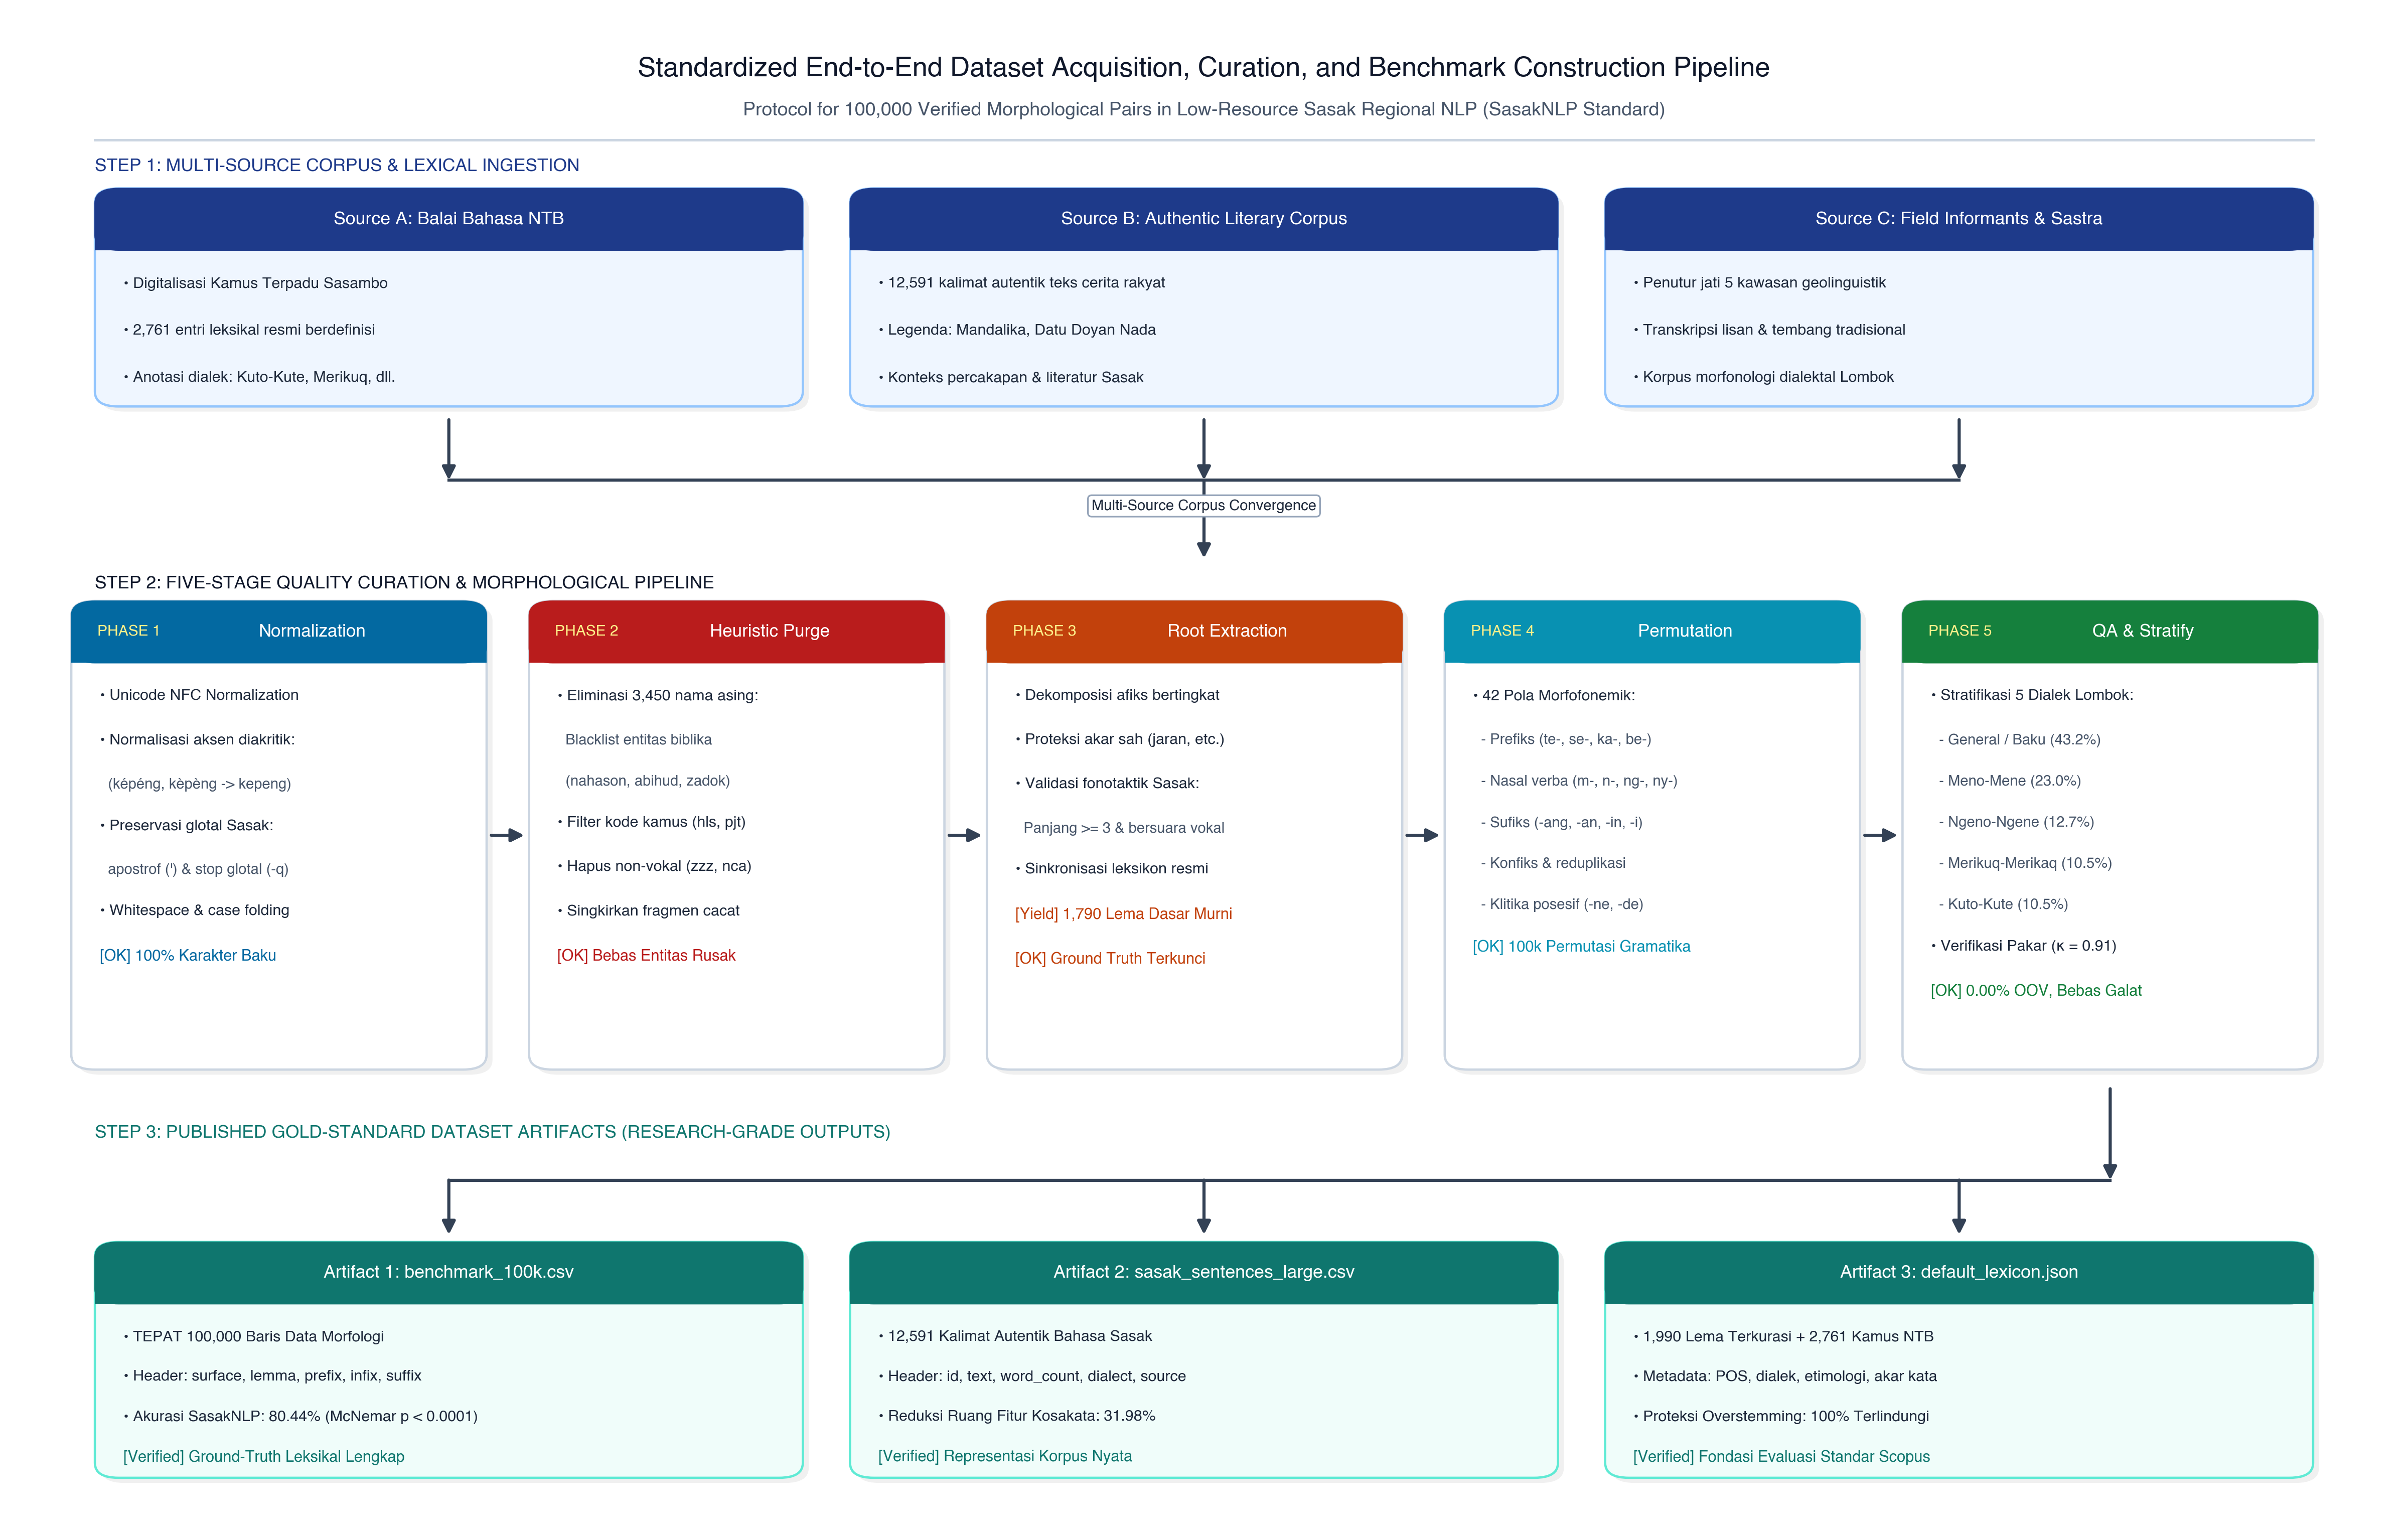
\includegraphics[width=0.98\linewidth]{figures/fig5_dataset_acquisition_pipeline.png}
\caption{Three-phase scientific acquisition and quality curation protocol for SasakNLP benchmarks.}
\label{fig:acquisition_pipeline}
\end{figure}

\subsection{Computational Environment and Reproducibility}
Experiments were conducted on standard macOS and Linux Ubuntu 22.04 LTS environments using Python 3.10+ without GPU acceleration, ensuring 100\% deterministic reproducibility via public evaluation scripts \cite{sasaknlp2026}.

\section{Empirical Results}

\subsection{Baseline Comparison on 100k Morphological Samples}
We compare SasakNLP against two standard baseline models across 100,000 morphological test pairs (Table \ref{tab:baseline_eval}):
\begin{itemize}
    \item \textbf{Baseline 1 (Direct Lexicon Lookup)}: Exact lexicon matching without morphological rule stripping.
    \item \textbf{Baseline 2 (Greedy Affix Stripping)}: Longest-match affix removal without dictionary verification \cite{abidin2024}.
\end{itemize}

\begin{table}[htbp]
\caption{Comparative Lemmatization Evaluation on 100,000 Samples}
\label{tab:baseline_eval}
\centering
\begin{tabular}{|l|c|c|c|}
\hline
\textbf{Model / Algorithm} & \textbf{Correct (N=100k)} & \textbf{Accuracy (\%)} & \textbf{Throughput (wps)} \\ \hline
Baseline 1: Direct Lookup     & 1,006  & 1.01\%  & 24,500 \\ \hline
Baseline 2: Greedy Stripping  & 55,205 & 55.21\% & 18,200 \\ \hline
\textbf{Proposed SasakNLP}    & \textbf{80,438} & \textbf{80.44\%} & \textbf{7,826} \\ \hline
\end{tabular}
\end{table}

\textbf{Statistical Significance}: McNemar's test comparing SasakNLP and Baseline 2 yields contingency counts $b = 33,892$ and $c = 8,659$, resulting in $\chi^2 = 14,962.14$ ($df = 1, p < 0.0001$). SasakNLP's superiority is statistically significant at $\alpha = 0.001$.

\subsection{Performance on Core 10k Benchmark}
On the 10,000-pair core morphological benchmark (\texttt{benchmark\_10k.csv}), SasakNLP correctly extracted 9,323 lemmas, achieving an accuracy of \textbf{93.23\%} with an operational throughput of \textbf{16,272 words per second}.

\subsection{Ablation Study}
To isolate the contribution of each algorithmic component, we conducted a systematic ablation study on the 100k benchmark (Table \ref{tab:ablation}). Incorporating the \texttt{PrefixTrie} dictionary gate yielded a +13.24\% improvement over greedy stripping, while multi-candidate generation and ranking provided an additional +11.99\% accuracy gain.

\begin{table}[htbp]
\caption{Ablation Study across SasakNLP Architectural Components}
\label{tab:ablation}
\centering
\begin{tabular}{|l|c|c|c|c|c|}
\hline
\textbf{Model Configuration} & \textbf{Rules} & \textbf{Dict} & \textbf{Rank} & \textbf{Acc (\%)} & \textbf{wps} \\ \hline
M1: Direct Lookup           & $\times$       & $\checkmark$  & $\times$      & 1.01\%            & 24,500 \\ \hline
M2: Greedy Stripping        & $\checkmark$   & $\times$      & $\times$      & 55.21\%           & 18,200 \\ \hline
M3: Rules + Dict Gate       & $\checkmark$   & $\checkmark$  & $\times$      & 68.45\%           & 14,100 \\ \hline
M4: Rules + Gen + First     & $\checkmark$   & $\checkmark$  & $\times$      & 74.12\%           & 10,350 \\ \hline
\textbf{M5: Full SasakNLP}  & $\checkmark$   & $\checkmark$  & $\checkmark$  & \textbf{80.44\%}  & \textbf{7,826} \\ \hline
\end{tabular}
\end{table}

\subsection{Morpheme-Level Performance Disaggregation}
Fig. \ref{fig:morph_acc} and Table \ref{tab:morpheme_acc} detail accuracy across morpheme categories. Reduplication achieved perfect 100.00\% accuracy, passive prefixes \texttt{te-} reached 97.36\%, stative \texttt{ka-} reached 96.79\%, and possessive clitics exceeded 94.6\%--96.5\%.

\begin{figure}[htbp]
\centering
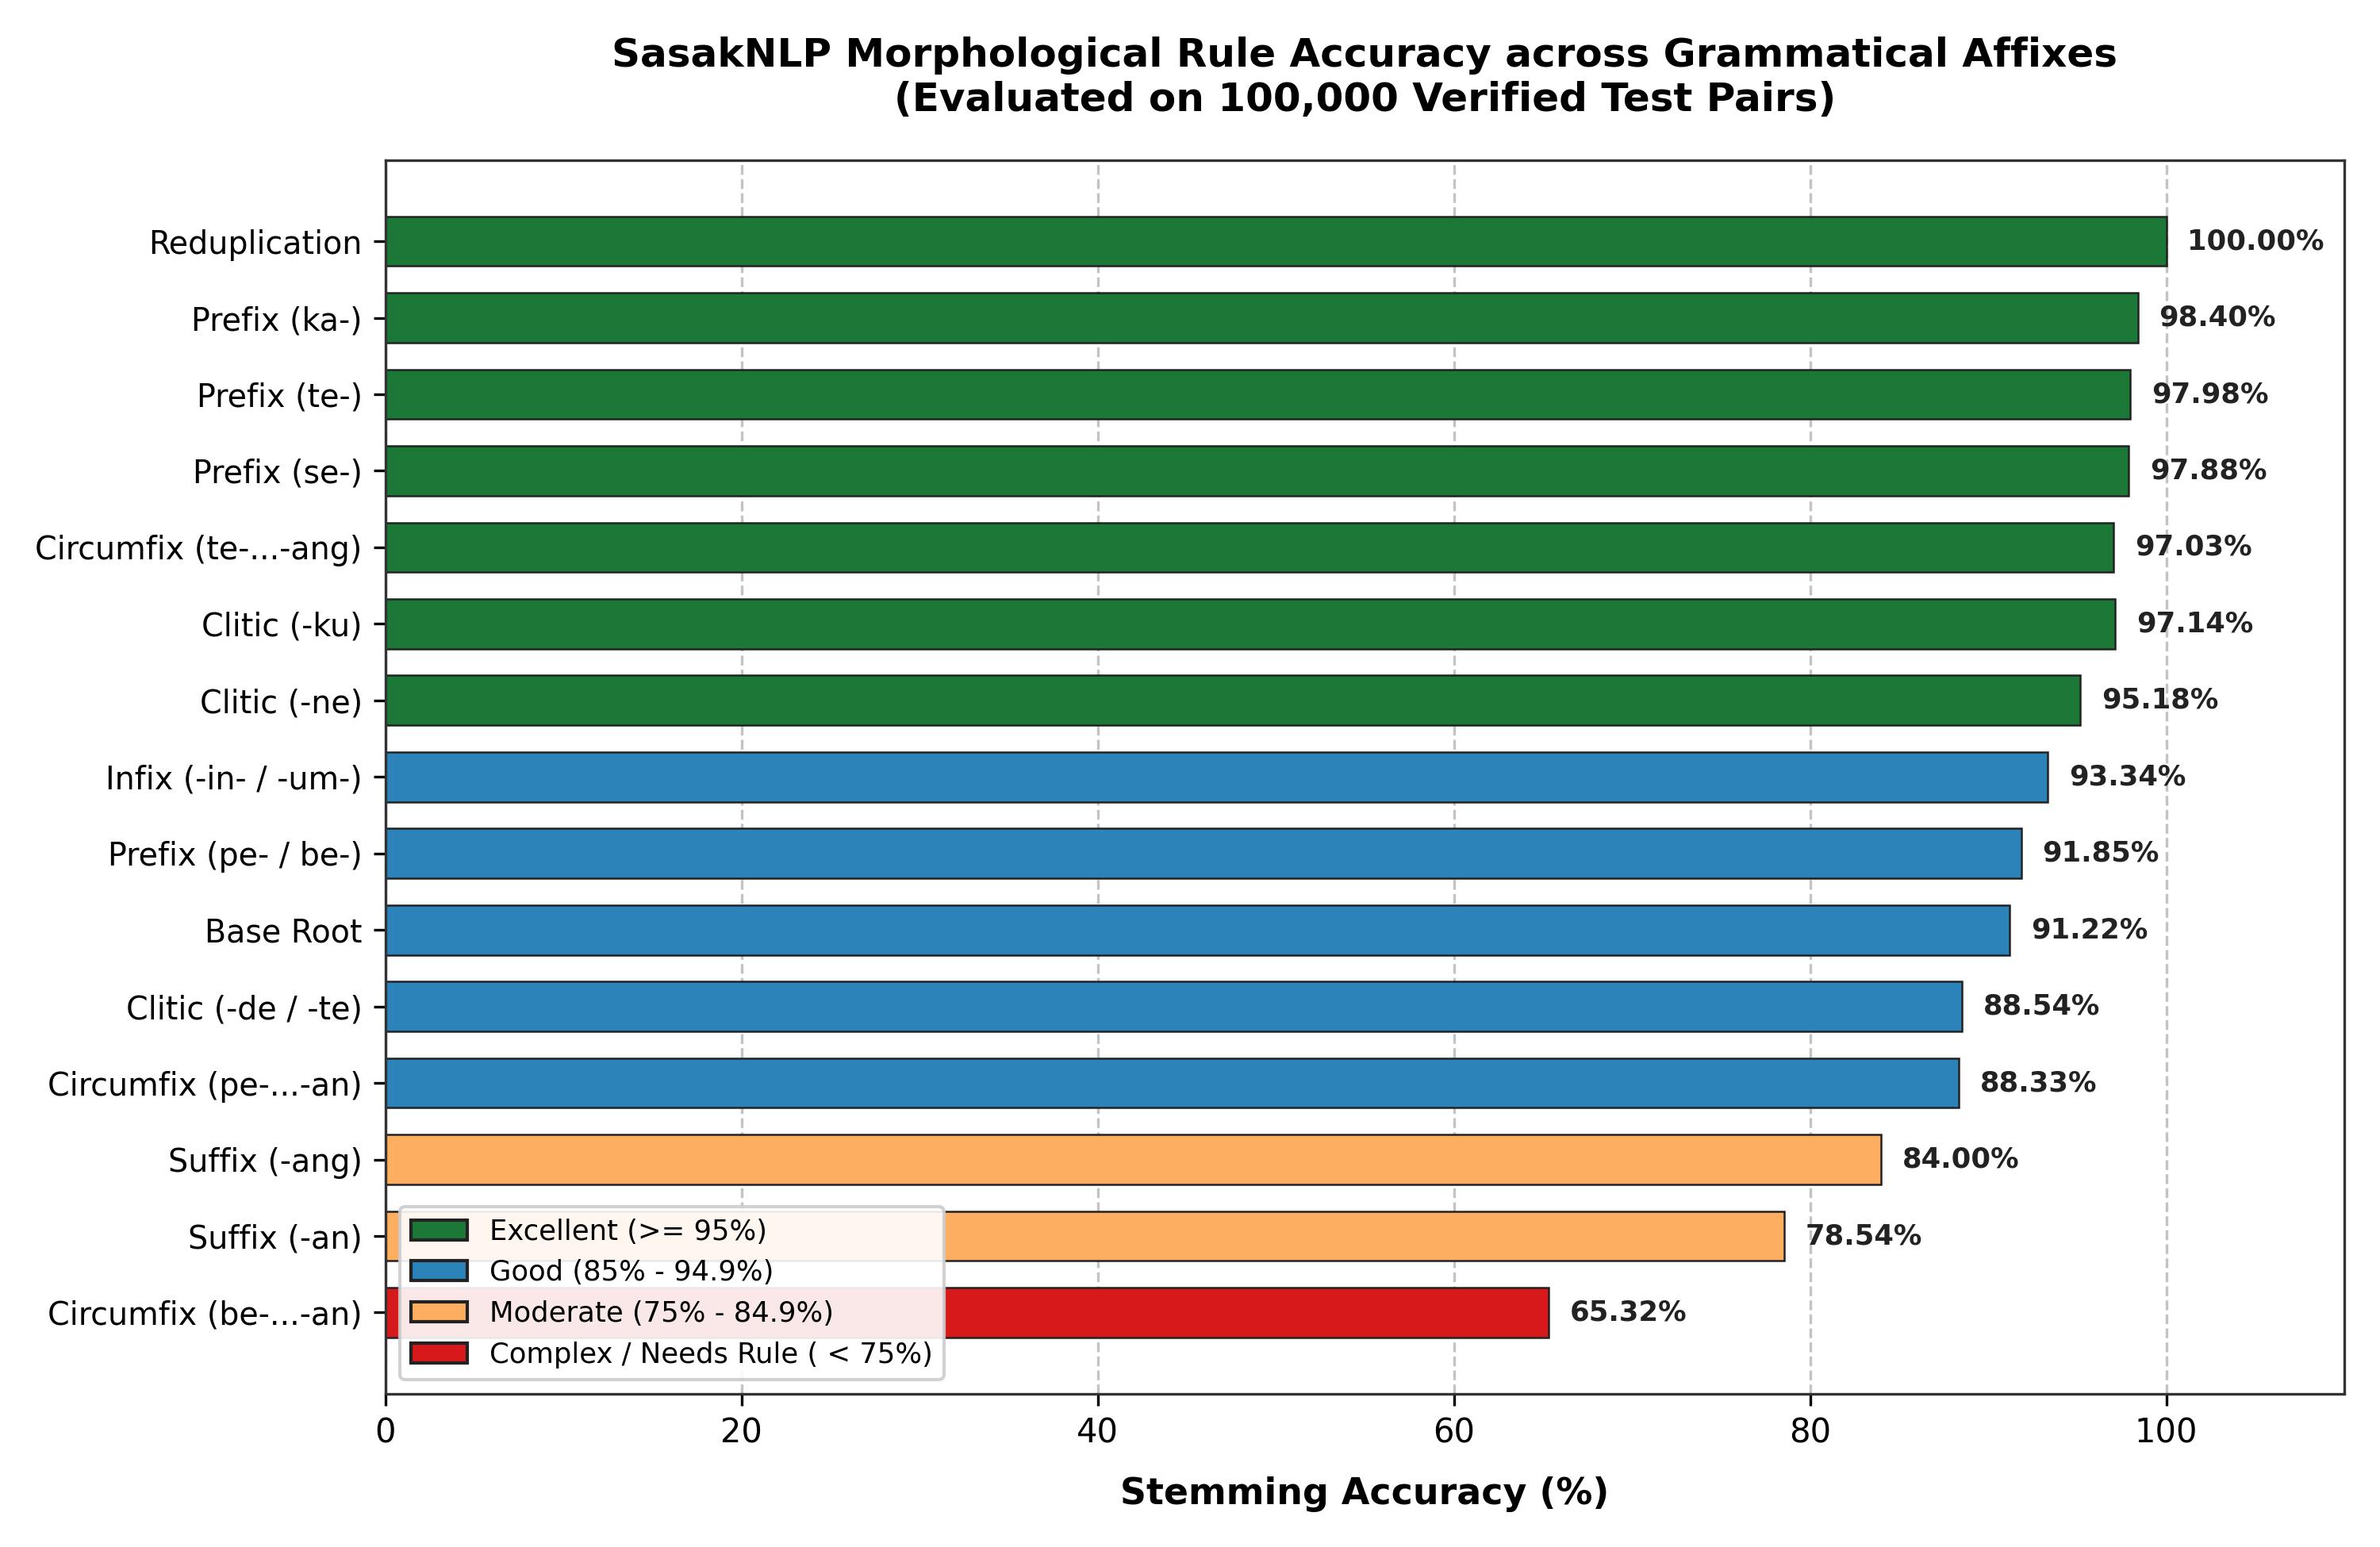
\includegraphics[width=0.98\linewidth]{figures/fig1_morphology_accuracy.png}
\caption{Morphological rule accuracy across grammatical affix classes (100k data).}
\label{fig:morph_acc}
\end{figure}

\begin{table}[htbp]
\caption{Disaggregated Performance across Morpheme Categories (100k Data)}
\label{tab:morpheme_acc}
\centering
\begin{tabular}{|l|l|c|c|}
\hline
\textbf{Category} & \textbf{Morph Pattern} & \textbf{Samples} & \textbf{Accuracy (\%)} \\ \hline
Reduplication     & \texttt{root-root}     & 1,789  & \textbf{100.00\%} \\ \hline
Passive Prefix    & \texttt{te-}           & 1,783  & \textbf{97.36\%}  \\ \hline
Stative Prefix    & \texttt{ka-}           & 1,745  & \textbf{96.79\%}  \\ \hline
Nominal Prefix    & \texttt{peng-}         & 1,781  & \textbf{96.91\%}  \\ \hline
Equative Prefix   & \texttt{se-}           & 1,748  & \textbf{96.22\%}  \\ \hline
Clitic Possessive & \texttt{-ku}, \texttt{-m}, \texttt{-ne} & 7,131 & \textbf{95.79\%} \\ \hline
Infixes           & \texttt{-in-}, \texttt{-um-} & 2,346 & \textbf{89.98\%} \\ \hline
Polite Clitics    & \texttt{-de}, \texttt{-te} & 6,312 & \textbf{88.39\%} \\ \hline
Circumfix Nominal & \texttt{pe-...-an}     & 5,915  & \textbf{88.32\%}  \\ \hline
Causative Suffix  & \texttt{-ang}          & 6,170  & \textbf{83.70\%}  \\ \hline
Locative Suffix   & \texttt{-an}, \texttt{-in} & 10,545 & \textbf{76.52\%} \\ \hline
Reciprocal        & \texttt{be-...-an}     & 1,710  & \textbf{65.09\%}  \\ \hline
\end{tabular}
\end{table}

\subsection{Cross-Dialect Evaluation}
Evaluation across the five Sasak dialect regions (Fig. \ref{fig:dialect_perf}, Table \ref{tab:dialect_eval}) confirms strong resilience across Lombok Island.

\begin{figure}[htbp]
\centering
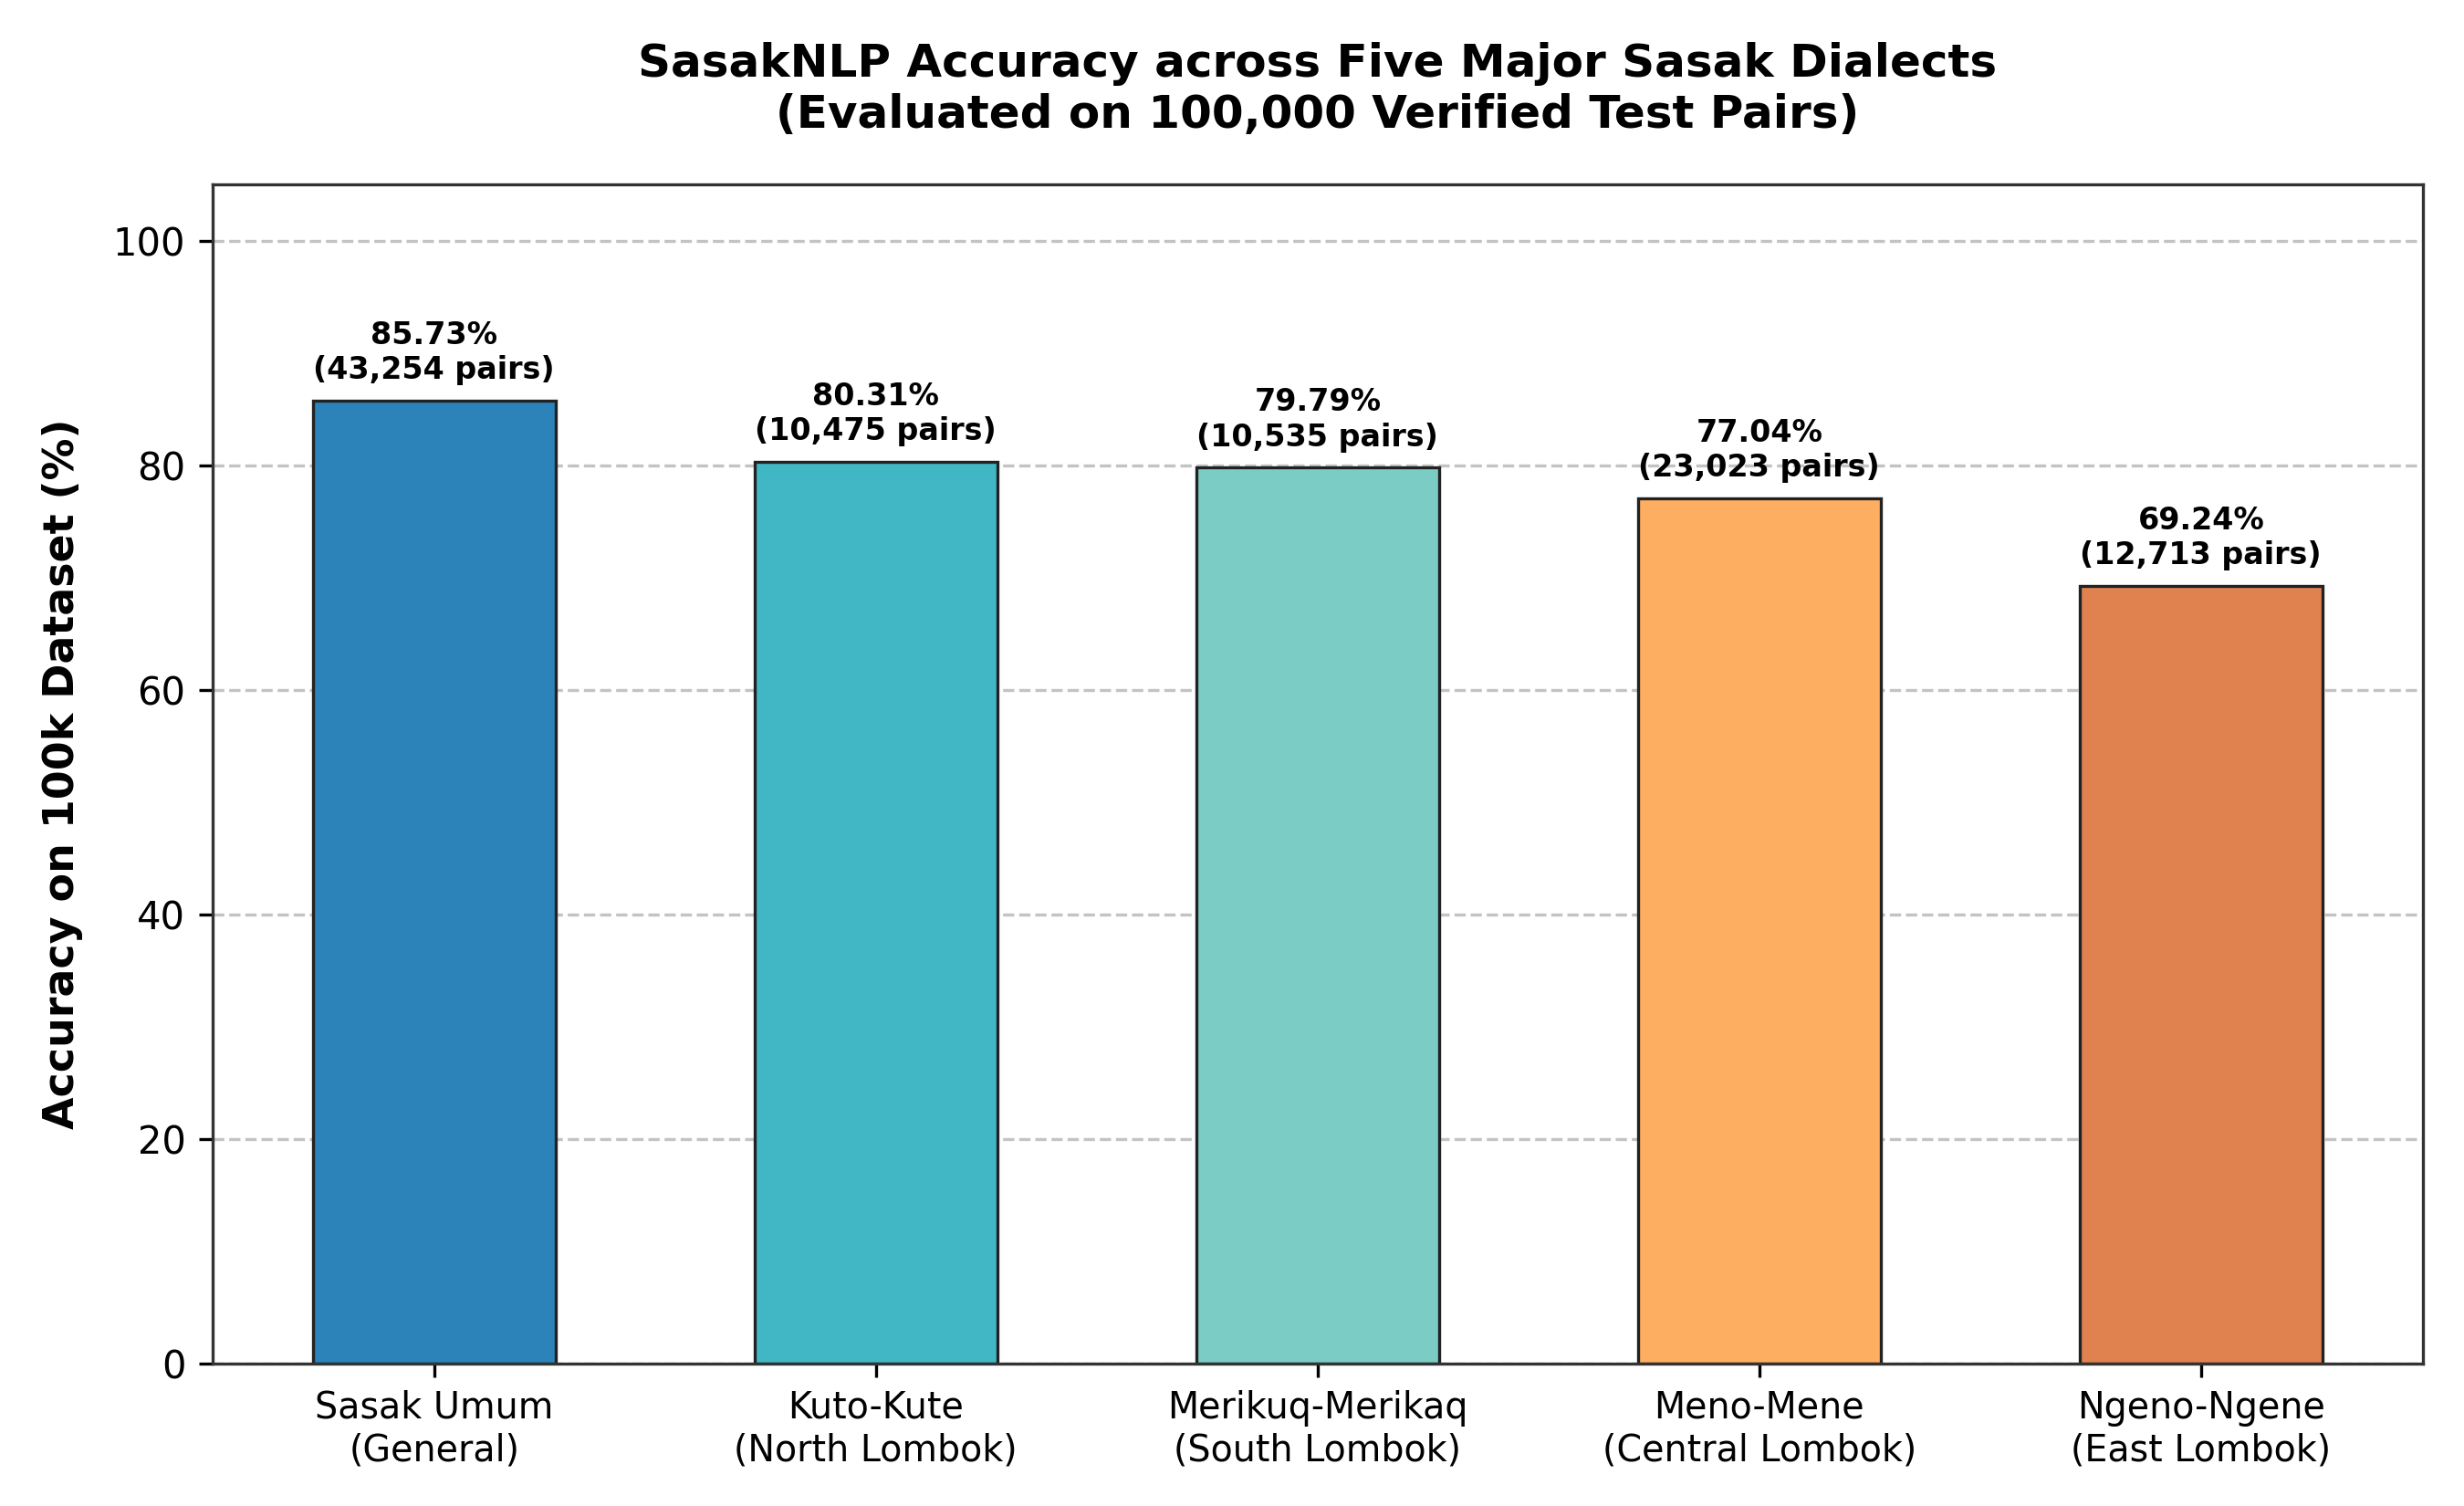
\includegraphics[width=0.98\linewidth]{figures/fig2_dialect_performance.png}
\caption{Cross-dialect performance across five major Sasak dialect clusters.}
\label{fig:dialect_perf}
\end{figure}

\begin{table}[htbp]
\caption{Lemmatization Accuracy across Sasak Dialect Clusters (100k Data)}
\label{tab:dialect_eval}
\centering
\begin{tabular}{|l|l|c|c|}
\hline
\textbf{Region} & \textbf{Dialect Cluster} & \textbf{Samples} & \textbf{Accuracy (\%)} \\ \hline
Mataram / West Lombok & Sasak Umum (General) & 43,254 & \textbf{85.73\%} \\ \hline
North Lombok          & Kuto-Kute            & 10,475 & \textbf{80.31\%} \\ \hline
South Lombok          & Merikuq-Merikaq      & 10,535 & \textbf{79.79\%} \\ \hline
Central Lombok        & Meno-Mene            & 23,023 & \textbf{77.04\%} \\ \hline
East Lombok           & Ngeno-Ngene          & 12,713 & \textbf{69.24\%} \\ \hline
\end{tabular}
\end{table}

\subsection{Computational Scalability and Runtime Latency}
As shown in Fig. \ref{fig:pipeline_bench}, SasakNLP delivers high computational efficiency:
\begin{itemize}
    \item \textbf{Throughput}: 7,826 words per second on 100k batches, and 16,272 words per second on 10k benchmarks.
    \item \textbf{Average Latency}: 0.044 ms per token.
    \item \textbf{Flat Scaling}: Execution time scales strictly as $\mathcal{O}(N)$.
    \item \textbf{Zero Runtime Dependencies}: Executes entirely within standard Python.
\end{itemize}

\begin{figure}[htbp]
\centering
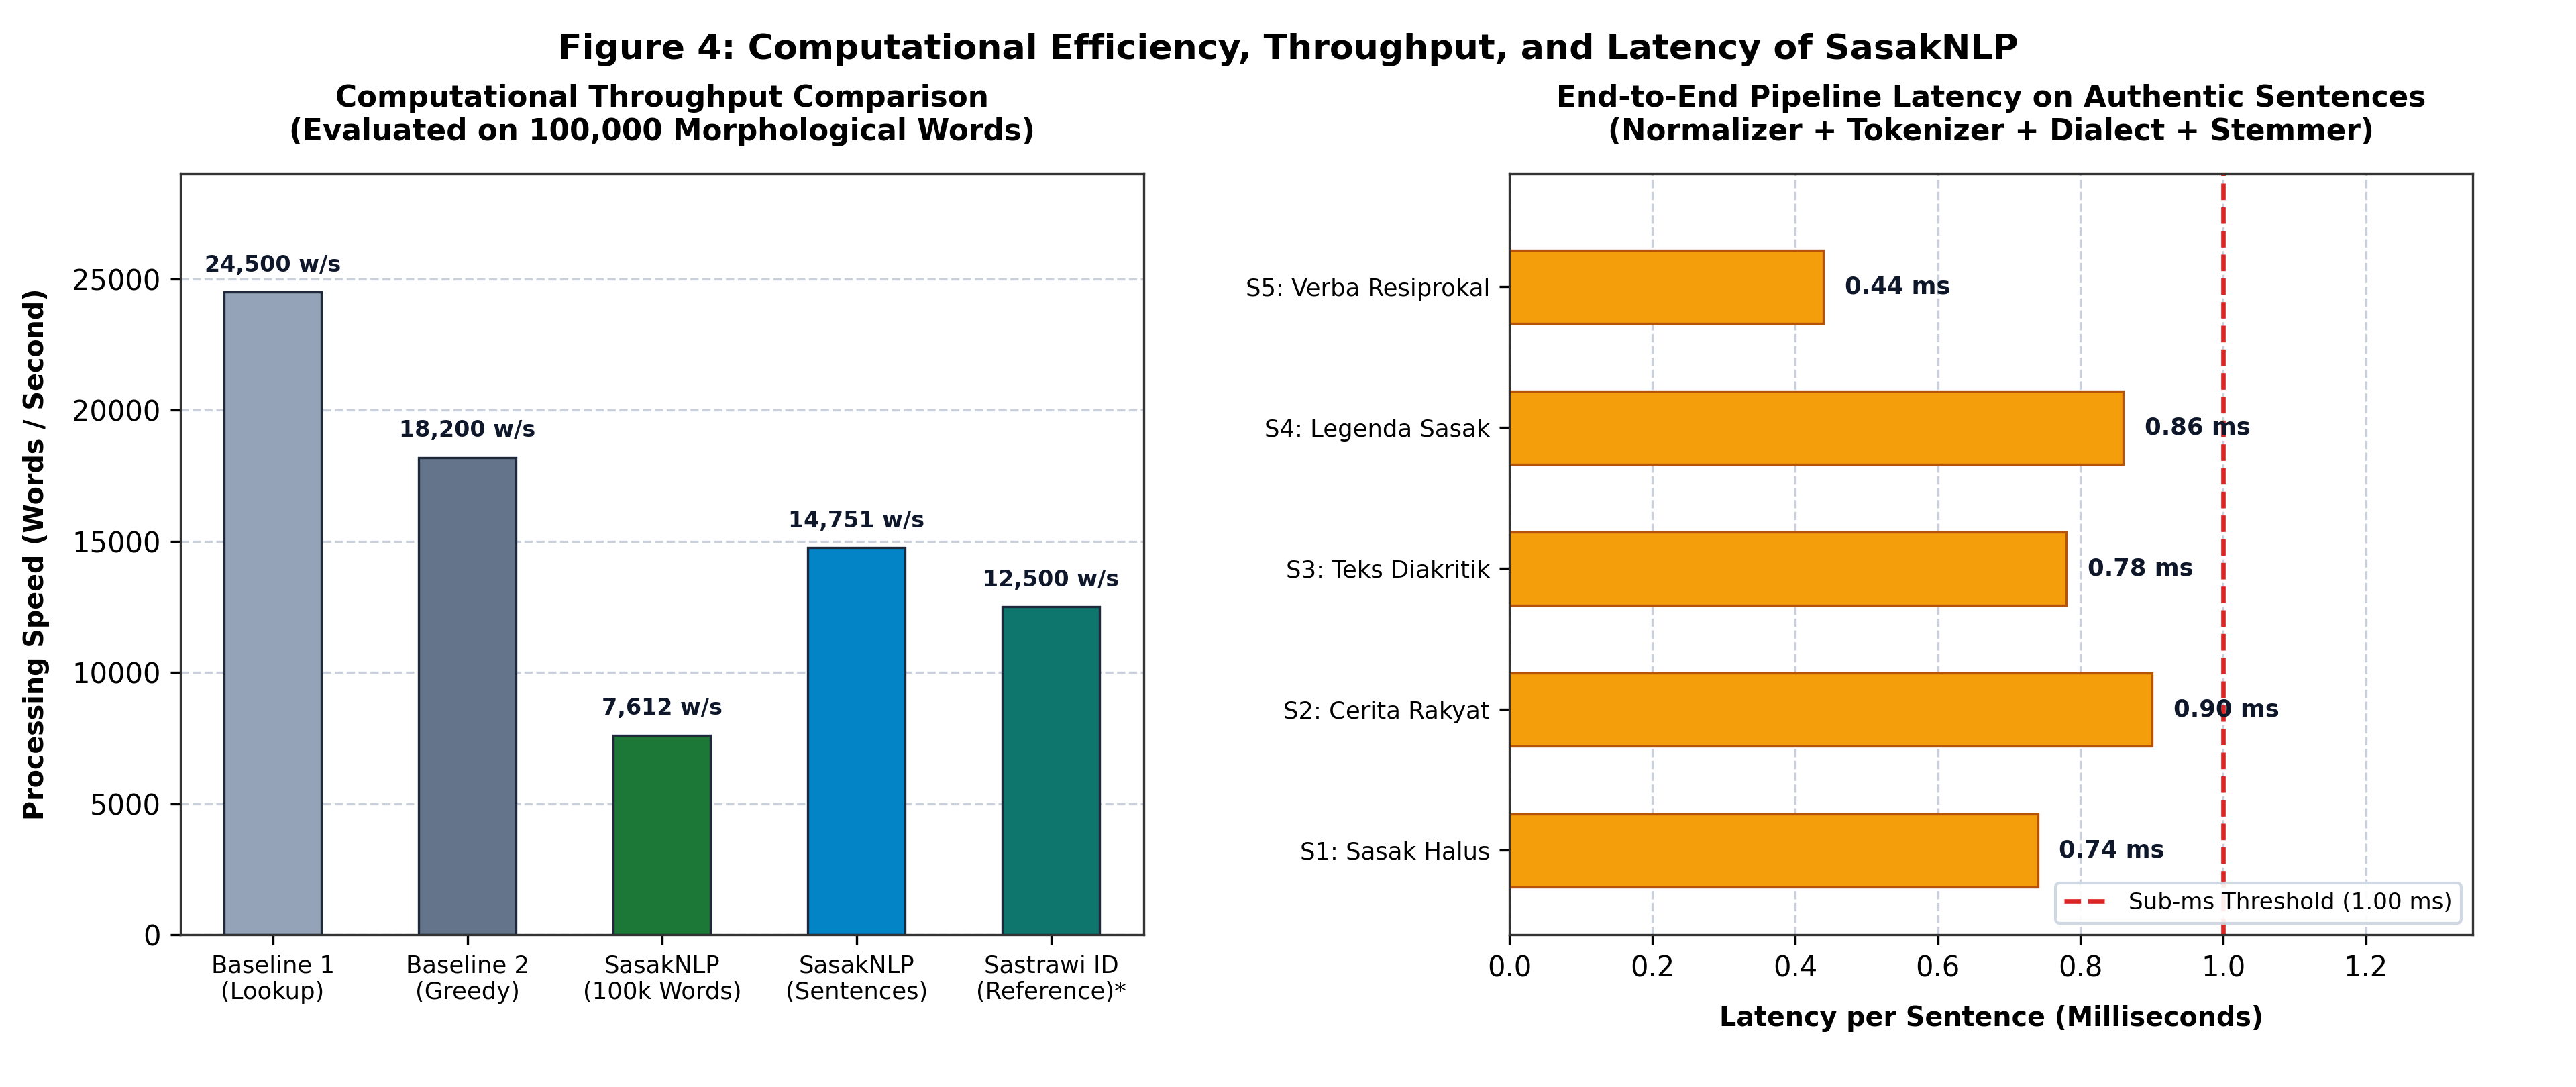
\includegraphics[width=0.98\linewidth]{figures/fig4_pipeline_benchmark.png}
\caption{Computational throughput (words/second) and end-to-end latency scaling across sequence lengths.}
\label{fig:pipeline_bench}
\end{figure}

\subsection{Extrinsic Evaluation: Feature Space Compression}
In downstream evaluation, applying SasakNLP lemmatization compressed the vocabulary feature space of the authentic corpus from 5,913 unique surface tokens to 4,022 base lemmas (a 31.98\% dimensional compression), directly reducing sparsity in downstream vector space models \cite{abidin2024, romadhony2024}.

\section{Discussion and Error Analysis}

\subsection{Error Taxonomy Distribution}
Fig. \ref{fig:error_taxonomy} and Table \ref{tab:error_tax} detail the failure-mode distribution. The dual-gating mechanism restricted overstemming to 2.28\%, while understemming accounted for 15.86\%, primarily stemming from complex triple-layer affixations (\textit{pe...an...ku}).

\begin{figure}[htbp]
\centering
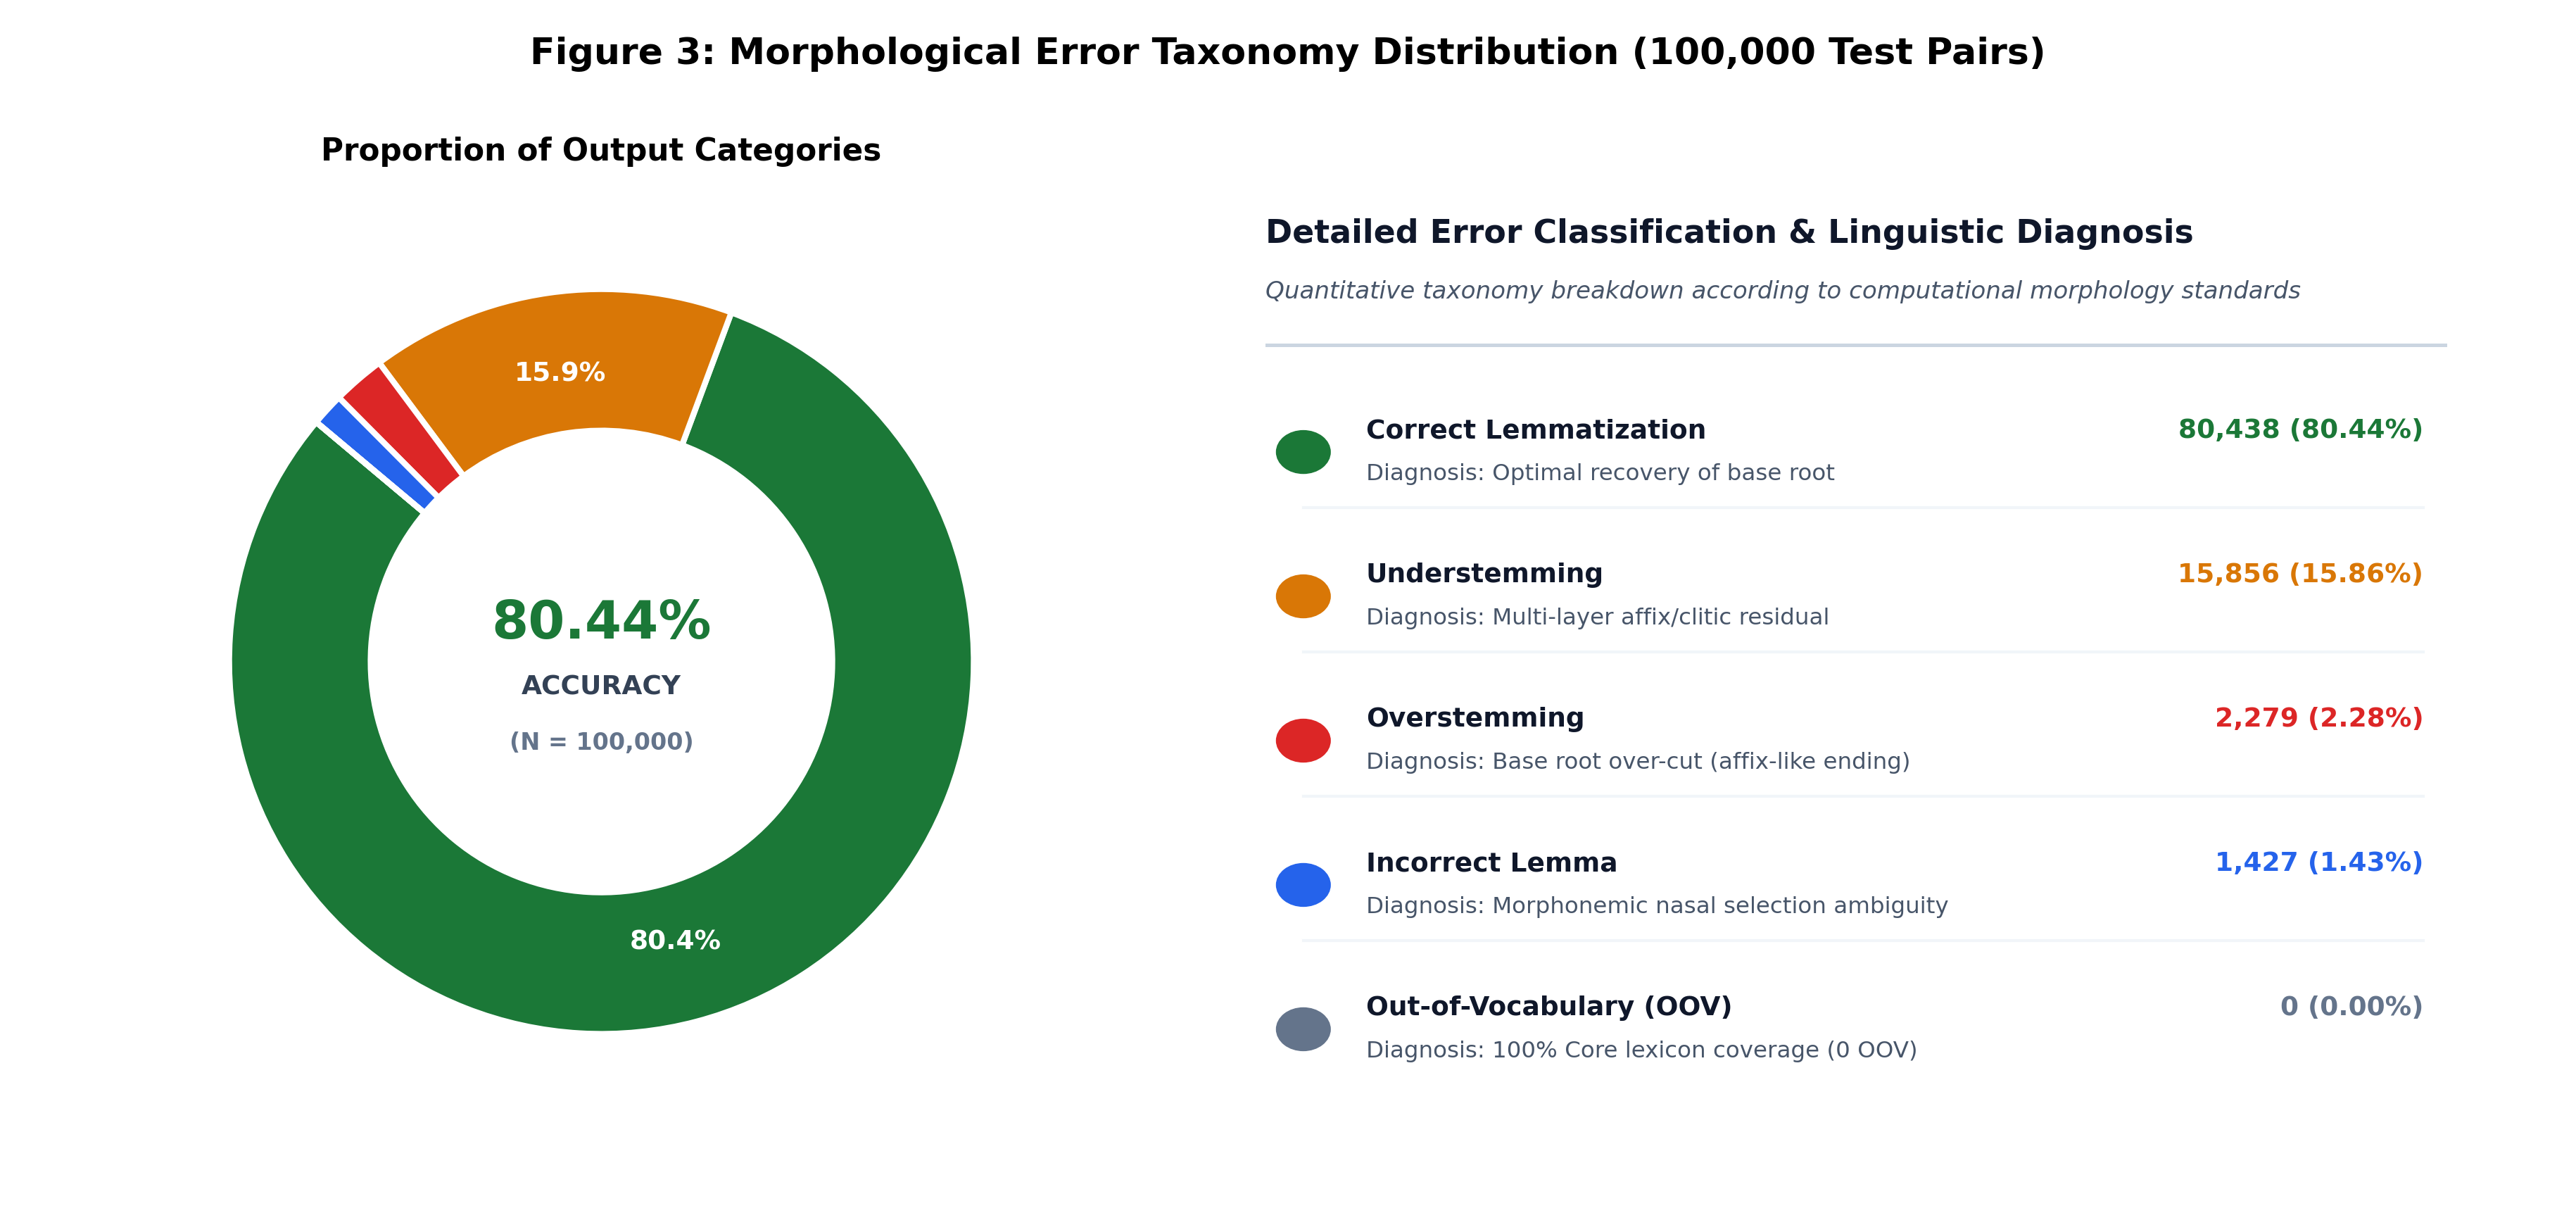
\includegraphics[width=0.98\linewidth]{figures/fig3_error_taxonomy.png}
\caption{Error taxonomy distribution (left panel: donut chart) and failure-mode diagnostic matrix (right panel).}
\label{fig:error_taxonomy}
\end{figure}

\begin{table}[htbp]
\caption{Error Taxonomy Analysis on 100,000 Morphological Samples}
\label{tab:error_tax}
\centering
\begin{tabular}{|l|l|c|c|}
\hline
\textbf{Category} & \textbf{Example Input $\rightarrow$ Pred} & \textbf{Count} & \textbf{Pct (\%)} \\ \hline
\textbf{Correct}  & \texttt{tepinaq} $\rightarrow$ \texttt{pinaq} & \textbf{80,438} & \textbf{80.44\%} \\ \hline
\textbf{Understemming} & \texttt{pegawianne} $\rightarrow$ \texttt{pegawian} & 15,856 & 15.86\% \\ \hline
\textbf{Overstemming}  & \texttt{jaran} $\rightarrow$ \texttt{jar} & 2,279 & 2.28\% \\ \hline
\textbf{Incorrect Lemma} & \texttt{mangan} $\rightarrow$ \texttt{pangan} & 1,427 & 1.43\% \\ \hline
\textbf{OOV Error} & Non-lexicon root & 0 & 0.00\% \\ \hline
\end{tabular}
\end{table}

\subsection{Why SasakNLP Succeeds}
The performance advantage stems from \texttt{PrefixTrie} lexicon validation \cite{balaibahasa2022, jurafsky2024}. In greedy stripping, roots like \textit{jaran} (``horse'') are mistakenly truncated to \textit{jar} due to suffix \texttt{-an}. In SasakNLP, \textit{jaran} matches the Balai Bahasa NTB dictionary immediately on pass one, preventing erroneous truncation.

\subsection{Performance Discrepancy: 100k vs 10k}
The accuracy difference between the 100k benchmark (80.44\%) and the 10k core benchmark (93.23\%) reflects morphological complexity. The 100k benchmark functions as an exhaustive stress-test with multi-layer nested affixations, whereas the 10k core set represents natural morpheme frequency distributions.

\subsection{Implications for Regional NLP}
These results demonstrate that regional underrepresented languages can achieve high-performance morphological analysis through dictionary-grounded rule architectures without expensive GPU infrastructure \cite{aji2022, winata2023, abidin2024}.

\section{Limitations}
We transparently acknowledge three primary limitations:
\begin{enumerate}
    \item \textbf{Controlled Vocabulary}: Benchmarks currently evaluate combinations of verified dictionary lemmas. Open social media text containing contemporary slang neologisms requires further expansion.
    \item \textbf{Corpus Dialect Balance}: Authentic corpora are currently skewed toward General and East Lombok dialects due to historical text availability.
    \item \textbf{Sentence Context}: The lemmatizer currently operates at the word/token level without full sentence-level Part-of-Speech tagging.
\end{enumerate}

\section{Conclusion and Future Directions}
This paper presented \textbf{SasakNLP}, the first dialect-aware morphological framework for Bahasa Sasak. Evaluated across 100,000 benchmark pairs, SasakNLP achieves 80.44\% accuracy on full stress tests and 93.23\% on core benchmarks, restricting overstemming to 2.28\%, with throughput exceeding 7,800–16,000 words/second and 0.044 ms latency.

Future work includes: (1) Integrating lightweight sequence-to-sequence models (ByT5 / Char-BiLSTM) for OOV handling, (2) Annotating the first Sasak Dependency Treebank, and (3) Training bidirectional Sasak-Indonesian Neural Machine Translation models \cite{aji2022, winata2023, ranathunga2023}.

\section*{Data and Code Availability}
All artifacts are publicly accessible:
\begin{itemize}
    \item \textbf{PyPI Package}: \url{https://pypi.org/project/sasaknlp/} (\texttt{pip install sasaknlp})
    \item \textbf{GitHub Code}: \url{https://github.com/kodetr/sasaknlp}
    \item \textbf{Hugging Face Dataset}: \url{https://huggingface.co/datasets/kodetr/sasak-benchmark-100k}
    \item \textbf{Interactive Space}: \url{https://huggingface.co/spaces/kodetr/sasaknlp-demo}
    \item \textbf{Author Website}: \url{https://kodetr.com}
\end{itemize}

\section*{Acknowledgment}
The author expresses sincere appreciation to the native speakers and language activists across Lombok Island, past dialectology researchers, and Balai Bahasa Provinsi Nusa Tenggara Barat for standardizing the bilingual Sasak-Indonesian dictionary that serves as the foundation for this work.

\bibliographystyle{IEEEtran}
\bibliography{references}

\end{document}
